\documentclass[twoside]{book}

% Packages required by doxygen
\usepackage{fixltx2e}
\usepackage{calc}
\usepackage{doxygen}
\usepackage[export]{adjustbox} % also loads graphicx
\usepackage{graphicx}
\usepackage[utf8]{inputenc}
\usepackage{makeidx}
\usepackage{multicol}
\usepackage{multirow}
\PassOptionsToPackage{warn}{textcomp}
\usepackage{textcomp}
\usepackage[nointegrals]{wasysym}
\usepackage[table]{xcolor}

% Font selection
\usepackage[T1]{fontenc}
\usepackage[scaled=.90]{helvet}
\usepackage{courier}
\usepackage{amssymb}
\usepackage{sectsty}
\renewcommand{\familydefault}{\sfdefault}
\allsectionsfont{%
  \fontseries{bc}\selectfont%
  \color{darkgray}%
}
\renewcommand{\DoxyLabelFont}{%
  \fontseries{bc}\selectfont%
  \color{darkgray}%
}
\newcommand{\+}{\discretionary{\mbox{\scriptsize$\hookleftarrow$}}{}{}}

% Page & text layout
\usepackage{geometry}
\geometry{%
  a4paper,%
  top=2.5cm,%
  bottom=2.5cm,%
  left=2.5cm,%
  right=2.5cm%
}
\tolerance=750
\hfuzz=15pt
\hbadness=750
\setlength{\emergencystretch}{15pt}
\setlength{\parindent}{0cm}
\setlength{\parskip}{3ex plus 2ex minus 2ex}
\makeatletter
\renewcommand{\paragraph}{%
  \@startsection{paragraph}{4}{0ex}{-1.0ex}{1.0ex}{%
    \normalfont\normalsize\bfseries\SS@parafont%
  }%
}
\renewcommand{\subparagraph}{%
  \@startsection{subparagraph}{5}{0ex}{-1.0ex}{1.0ex}{%
    \normalfont\normalsize\bfseries\SS@subparafont%
  }%
}
\makeatother

% Headers & footers
\usepackage{fancyhdr}
\pagestyle{fancyplain}
\fancyhead[LE]{\fancyplain{}{\bfseries\thepage}}
\fancyhead[CE]{\fancyplain{}{}}
\fancyhead[RE]{\fancyplain{}{\bfseries\leftmark}}
\fancyhead[LO]{\fancyplain{}{\bfseries\rightmark}}
\fancyhead[CO]{\fancyplain{}{}}
\fancyhead[RO]{\fancyplain{}{\bfseries\thepage}}
\fancyfoot[LE]{\fancyplain{}{}}
\fancyfoot[CE]{\fancyplain{}{}}
\fancyfoot[RE]{\fancyplain{}{\bfseries\scriptsize Generated by Doxygen }}
\fancyfoot[LO]{\fancyplain{}{\bfseries\scriptsize Generated by Doxygen }}
\fancyfoot[CO]{\fancyplain{}{}}
\fancyfoot[RO]{\fancyplain{}{}}
\renewcommand{\footrulewidth}{0.4pt}
\renewcommand{\chaptermark}[1]{%
  \markboth{#1}{}%
}
\renewcommand{\sectionmark}[1]{%
  \markright{\thesection\ #1}%
}

% Indices & bibliography
\usepackage{natbib}
\usepackage[titles]{tocloft}
\setcounter{tocdepth}{3}
\setcounter{secnumdepth}{5}
\makeindex

% Hyperlinks (required, but should be loaded last)
\usepackage{ifpdf}
\ifpdf
  \usepackage[pdftex,pagebackref=true]{hyperref}
\else
  \usepackage[ps2pdf,pagebackref=true]{hyperref}
\fi
\hypersetup{%
  colorlinks=true,%
  linkcolor=blue,%
  citecolor=blue,%
  unicode%
}

% Custom commands
\newcommand{\clearemptydoublepage}{%
  \newpage{\pagestyle{empty}\cleardoublepage}%
}

\usepackage{caption}
\captionsetup{labelsep=space,justification=centering,font={bf},singlelinecheck=off,skip=4pt,position=top}

%===== C O N T E N T S =====

\begin{document}

% Titlepage & ToC
\hypersetup{pageanchor=false,
             bookmarksnumbered=true,
             pdfencoding=unicode
            }
\pagenumbering{roman}
\begin{titlepage}
\vspace*{7cm}
\begin{center}%
{\Large Kitting Cell }\\
\vspace*{1cm}
{\large Generated by Doxygen 1.8.11}\\
\end{center}
\end{titlepage}
\clearemptydoublepage
\tableofcontents
\clearemptydoublepage
\pagenumbering{arabic}
\hypersetup{pageanchor=true}

%--- Begin generated contents ---
\chapter{Class Index}
\section{Class List}
Here are the classes, structs, unions and interfaces with brief descriptions\+:\begin{DoxyCompactList}
\item\contentsline{section}{\hyperlink{classGrip}{Grip} }{\pageref{classGrip}}{}
\item\contentsline{section}{\hyperlink{classkuka}{kuka} \\*Class to calculate forward and inverse kinematics for K\+U\+KA I\+I\+WA }{\pageref{classkuka}}{}
\item\contentsline{section}{\hyperlink{classPerception}{Perception} }{\pageref{classPerception}}{}
\end{DoxyCompactList}

\chapter{File Index}
\section{File List}
Here is a list of all documented files with brief descriptions\+:\begin{DoxyCompactList}
\item\contentsline{section}{include/kitting\+\_\+cell/{\bfseries Grip.\+hpp} }{\pageref{Grip_8hpp}}{}
\item\contentsline{section}{include/kitting\+\_\+cell/\hyperlink{kuka_8hpp}{kuka.\+hpp} \\*This file defines the methods for class \char`\"{}kuka\char`\"{} to control a K\+U\+KA I\+I\+WA manipulator using on I\+I\+W\+A\+\_\+\+S\+T\+A\+CK using O\+R\+O\+C\+OS K\+DL }{\pageref{kuka_8hpp}}{}
\item\contentsline{section}{include/kitting\+\_\+cell/\hyperlink{Perception_8hpp}{Perception.\+hpp} \\*This file defines the methods for class the \hyperlink{classPerception}{Perception} class. This class is responsible for detection and localizing red, green, and blue objects in the image which is read through a R\+OS topic }{\pageref{Perception_8hpp}}{}
\item\contentsline{section}{src/\hyperlink{Grip_8cpp}{Grip.\+cpp} \\*This file defines methods for the \hyperlink{classGrip}{Grip} class. This class is used to toggle the vacuum gripper on a manipulator }{\pageref{Grip_8cpp}}{}
\item\contentsline{section}{src/\hyperlink{kuka_8cpp}{kuka.\+cpp} \\*This file implements the methods for class \char`\"{}kuka\char`\"{} This class cpp file defines data members and methods applicable for class kuka to to control a K\+U\+KA I\+I\+WA manipulator using on I\+I\+W\+A\+\_\+\+S\+T\+A\+CK using O\+R\+O\+C\+OS K\+DL for forward and inverse kinematics }{\pageref{kuka_8cpp}}{}
\item\contentsline{section}{test/\hyperlink{GripTests_8cpp}{Grip\+Tests.\+cpp} \\*This file defines the rostests and getests for \hyperlink{classGrip}{Grip} class }{\pageref{GripTests_8cpp}}{}
\item\contentsline{section}{test/\hyperlink{kukaTests_8cpp}{kuka\+Tests.\+cpp} \\*This is the file for testing the methods of the kuka class }{\pageref{kukaTests_8cpp}}{}
\item\contentsline{section}{test/\hyperlink{PerceptionTests_8cpp}{Perception\+Tests.\+cpp} \\*This is the file for testing the methods of the \hyperlink{classPerception}{Perception} class }{\pageref{PerceptionTests_8cpp}}{}
\end{DoxyCompactList}

\chapter{Class Documentation}
\hypertarget{classGrip}{}\section{Grip Class Reference}
\label{classGrip}\index{Grip@{Grip}}
\subsection*{Public Member Functions}
\begin{DoxyCompactItemize}
\item 
bool {\bfseries Toggle\+State} (bool)\hypertarget{classGrip_ad184a5badf82fce0514c1a6d8f9667f2}{}\label{classGrip_ad184a5badf82fce0514c1a6d8f9667f2}

\end{DoxyCompactItemize}


The documentation for this class was generated from the following files\+:\begin{DoxyCompactItemize}
\item 
include/kitting\+\_\+cell/Grip.\+hpp\item 
src/\hyperlink{Grip_8cpp}{Grip.\+cpp}\end{DoxyCompactItemize}

\hypertarget{classkuka}{}\section{kuka Class Reference}
\label{classkuka}\index{kuka@{kuka}}


Class to calculate forward and inverse kinematics for K\+U\+KA I\+I\+WA.  




{\ttfamily \#include $<$kuka.\+hpp$>$}

\subsection*{Public Member Functions}
\begin{DoxyCompactItemize}
\item 
\hyperlink{classkuka_af3a4e7638d63816706f342ddd9ca43e6}{kuka} ()\hypertarget{classkuka_af3a4e7638d63816706f342ddd9ca43e6}{}\label{classkuka_af3a4e7638d63816706f342ddd9ca43e6}

\begin{DoxyCompactList}\small\item\em This is the constructor for the class. \end{DoxyCompactList}\item 
trajectory\+\_\+msgs\+::\+Joint\+Trajectory \hyperlink{classkuka_a86a4b26cfec17bf0919ac8758768b9c1}{initialize\+Trajectory\+Point} ()
\begin{DoxyCompactList}\small\item\em This initializes kuka\+::joint\+Commands\+\_\+ to 0.\+0. \end{DoxyCompactList}\item 
trajectory\+\_\+msgs\+::\+Joint\+Trajectory\+Point \hyperlink{classkuka_afcf7e69ed9ef7a1a51f830ccaf320a4e}{initialize\+Home\+Pos} ()
\begin{DoxyCompactList}\small\item\em This initializes the home position for the robot. \end{DoxyCompactList}\item 
sensor\+\_\+msgs\+::\+Joint\+State \hyperlink{classkuka_a5ce8db8405b7decbad3ba449a7ad3731}{initialize\+Joints\+Sub} ()
\begin{DoxyCompactList}\small\item\em This initializes the variable that takes in the joint values from the subscriber. \end{DoxyCompactList}\item 
K\+D\+L\+::\+Jnt\+Array \hyperlink{classkuka_a12f118ede95479585988f4b25a67fb17}{initialize\+Joints\+K\+DL} ()
\begin{DoxyCompactList}\small\item\em This initializes the joint arrays that are fed to the kinematic solvers. \end{DoxyCompactList}\item 
K\+D\+L\+::\+Chain \hyperlink{classkuka_ab3c278ba250c7eda435f8dd801b5aca6}{make\+Chain} ()
\begin{DoxyCompactList}\small\item\em This defines the kinematic chain for K\+DL. \end{DoxyCompactList}\item 
trajectory\+\_\+msgs\+::\+Joint\+Trajectory\+Point \hyperlink{classkuka_ab1139c7fec434a2f8fa80f9358a5c9bc}{normalize\+Points} (K\+D\+L\+::\+Jnt\+Array)
\begin{DoxyCompactList}\small\item\em This normalizes the joint angles after Inverse Kinematics. \end{DoxyCompactList}\item 
void \hyperlink{classkuka_ab7ce79e8daaf42e58c7427c6ea885b59}{get\+Joints} (const sensor\+\_\+msgs\+::\+Joint\+State\+::\+Const\+Ptr \&joints\+State\+\_\+)
\begin{DoxyCompactList}\small\item\em This is the subscriber to read joint values for the robot. \end{DoxyCompactList}\item 
K\+D\+L\+::\+Jnt\+Array \hyperlink{classkuka_a3075c7d636fbc0f0d5629492a369c23a}{eval\+Kinematics\+IK} (K\+D\+L\+::\+Frame)
\begin{DoxyCompactList}\small\item\em This performs the inverse kinematics to get joint angles from cartesian pose. \end{DoxyCompactList}\item 
K\+D\+L\+::\+Frame \hyperlink{classkuka_a8886abcfe2aaf33b778a88834f03d6b6}{eval\+Kinematics\+FK} ()
\begin{DoxyCompactList}\small\item\em This performs the forward kinematics to get cartesian pose from joint angles. \end{DoxyCompactList}\item 
unsigned int \hyperlink{classkuka_a6c6f27f87873fd6d444e1f9878c36c93}{get\+Joint\+Nums} ()
\begin{DoxyCompactList}\small\item\em This calculates the number of joints in the chain and also preallocates joint\+Pos\+Kdl\+\_\+ and new\+Joint\+Pos\+Kdl\+\_\+ data members. \end{DoxyCompactList}\item 
trajectory\+\_\+msgs\+::\+Joint\+Trajectory \hyperlink{classkuka_af7cb1ea174f84bc7a38cb3196396e266}{drive\+Robot} (trajectory\+\_\+msgs\+::\+Joint\+Trajectory\+Point)
\begin{DoxyCompactList}\small\item\em This forms the Joint\+Trajectory message to whoch the robot is supposed to move. \end{DoxyCompactList}\item 
K\+D\+L\+::\+Jnt\+Array \hyperlink{classkuka_a44a8b59602c01cbf7606410871de7266}{return\+Curr\+Joints} ()
\begin{DoxyCompactList}\small\item\em This returns the current joint of the robot. \end{DoxyCompactList}\end{DoxyCompactItemize}


\subsection{Detailed Description}
Class to calculate forward and inverse kinematics for K\+U\+KA I\+I\+WA. 

\subsection{Member Function Documentation}
\index{kuka@{kuka}!drive\+Robot@{drive\+Robot}}
\index{drive\+Robot@{drive\+Robot}!kuka@{kuka}}
\subsubsection[{\texorpdfstring{drive\+Robot(trajectory\+\_\+msgs\+::\+Joint\+Trajectory\+Point)}{driveRobot(trajectory_msgs::JointTrajectoryPoint)}}]{\setlength{\rightskip}{0pt plus 5cm}trajectory\+\_\+msgs\+::\+Joint\+Trajectory kuka\+::drive\+Robot (
\begin{DoxyParamCaption}
\item[{trajectory\+\_\+msgs\+::\+Joint\+Trajectory\+Point}]{point}
\end{DoxyParamCaption}
)}\hypertarget{classkuka_af7cb1ea174f84bc7a38cb3196396e266}{}\label{classkuka_af7cb1ea174f84bc7a38cb3196396e266}


This forms the Joint\+Trajectory message to whoch the robot is supposed to move. 


\begin{DoxyParams}{Parameters}
{\em Joint\+Trajectory\+Point} & containing joint angles \\
\hline
\end{DoxyParams}
\begin{DoxyReturn}{Returns}
Joint\+Trajectory to drive the robot 
\end{DoxyReturn}
\index{kuka@{kuka}!eval\+Kinematics\+FK@{eval\+Kinematics\+FK}}
\index{eval\+Kinematics\+FK@{eval\+Kinematics\+FK}!kuka@{kuka}}
\subsubsection[{\texorpdfstring{eval\+Kinematics\+F\+K()}{evalKinematicsFK()}}]{\setlength{\rightskip}{0pt plus 5cm}K\+D\+L\+::\+Frame kuka\+::eval\+Kinematics\+FK (
\begin{DoxyParamCaption}
{}
\end{DoxyParamCaption}
)}\hypertarget{classkuka_a8886abcfe2aaf33b778a88834f03d6b6}{}\label{classkuka_a8886abcfe2aaf33b778a88834f03d6b6}


This performs the forward kinematics to get cartesian pose from joint angles. 


\begin{DoxyParams}{Parameters}
{\em none} & \\
\hline
\end{DoxyParams}
\begin{DoxyReturn}{Returns}
K\+D\+L\+::\+Frame type cartesian pose from FK 
\end{DoxyReturn}
\index{kuka@{kuka}!eval\+Kinematics\+IK@{eval\+Kinematics\+IK}}
\index{eval\+Kinematics\+IK@{eval\+Kinematics\+IK}!kuka@{kuka}}
\subsubsection[{\texorpdfstring{eval\+Kinematics\+I\+K(\+K\+D\+L\+::\+Frame)}{evalKinematicsIK(KDL::Frame)}}]{\setlength{\rightskip}{0pt plus 5cm}K\+D\+L\+::\+Jnt\+Array kuka\+::eval\+Kinematics\+IK (
\begin{DoxyParamCaption}
\item[{K\+D\+L\+::\+Frame}]{cartpos}
\end{DoxyParamCaption}
)}\hypertarget{classkuka_a3075c7d636fbc0f0d5629492a369c23a}{}\label{classkuka_a3075c7d636fbc0f0d5629492a369c23a}


This performs the inverse kinematics to get joint angles from cartesian pose. 


\begin{DoxyParams}{Parameters}
{\em the} & cartesian pose \\
\hline
\end{DoxyParams}
\begin{DoxyReturn}{Returns}
K\+D\+L\+::\+Jnt\+Array type joint array calculated from IK 
\end{DoxyReturn}
\index{kuka@{kuka}!get\+Joint\+Nums@{get\+Joint\+Nums}}
\index{get\+Joint\+Nums@{get\+Joint\+Nums}!kuka@{kuka}}
\subsubsection[{\texorpdfstring{get\+Joint\+Nums()}{getJointNums()}}]{\setlength{\rightskip}{0pt plus 5cm}unsigned int kuka\+::get\+Joint\+Nums (
\begin{DoxyParamCaption}
{}
\end{DoxyParamCaption}
)}\hypertarget{classkuka_a6c6f27f87873fd6d444e1f9878c36c93}{}\label{classkuka_a6c6f27f87873fd6d444e1f9878c36c93}


This calculates the number of joints in the chain and also preallocates joint\+Pos\+Kdl\+\_\+ and new\+Joint\+Pos\+Kdl\+\_\+ data members. 


\begin{DoxyParams}{Parameters}
{\em none} & \\
\hline
\end{DoxyParams}
\begin{DoxyReturn}{Returns}
number of joints as unsigned int variable 
\end{DoxyReturn}
\index{kuka@{kuka}!get\+Joints@{get\+Joints}}
\index{get\+Joints@{get\+Joints}!kuka@{kuka}}
\subsubsection[{\texorpdfstring{get\+Joints(const sensor\+\_\+msgs\+::\+Joint\+State\+::\+Const\+Ptr \&joints\+State\+\_\+)}{getJoints(const sensor_msgs::JointState::ConstPtr &jointsState_)}}]{\setlength{\rightskip}{0pt plus 5cm}void kuka\+::get\+Joints (
\begin{DoxyParamCaption}
\item[{const sensor\+\_\+msgs\+::\+Joint\+State\+::\+Const\+Ptr \&}]{joints\+State\+\_\+}
\end{DoxyParamCaption}
)}\hypertarget{classkuka_ab7ce79e8daaf42e58c7427c6ea885b59}{}\label{classkuka_ab7ce79e8daaf42e58c7427c6ea885b59}


This is the subscriber to read joint values for the robot. 


\begin{DoxyParams}{Parameters}
{\em joints\+State\+\_\+} & is the variable that holds the current joint values \\
\hline
\end{DoxyParams}
\begin{DoxyReturn}{Returns}
void 
\end{DoxyReturn}
\index{kuka@{kuka}!initialize\+Home\+Pos@{initialize\+Home\+Pos}}
\index{initialize\+Home\+Pos@{initialize\+Home\+Pos}!kuka@{kuka}}
\subsubsection[{\texorpdfstring{initialize\+Home\+Pos()}{initializeHomePos()}}]{\setlength{\rightskip}{0pt plus 5cm}trajectory\+\_\+msgs\+::\+Joint\+Trajectory\+Point kuka\+::initialize\+Home\+Pos (
\begin{DoxyParamCaption}
{}
\end{DoxyParamCaption}
)}\hypertarget{classkuka_afcf7e69ed9ef7a1a51f830ccaf320a4e}{}\label{classkuka_afcf7e69ed9ef7a1a51f830ccaf320a4e}


This initializes the home position for the robot. 


\begin{DoxyParams}{Parameters}
{\em none} & \\
\hline
\end{DoxyParams}
\begin{DoxyReturn}{Returns}
trajectory\+\_\+msgs\+::\+Joint\+Trajectory\+Point type variable to define robot\textquotesingle{}s destination 
\end{DoxyReturn}
\index{kuka@{kuka}!initialize\+Joints\+K\+DL@{initialize\+Joints\+K\+DL}}
\index{initialize\+Joints\+K\+DL@{initialize\+Joints\+K\+DL}!kuka@{kuka}}
\subsubsection[{\texorpdfstring{initialize\+Joints\+K\+D\+L()}{initializeJointsKDL()}}]{\setlength{\rightskip}{0pt plus 5cm}K\+D\+L\+::\+Jnt\+Array kuka\+::initialize\+Joints\+K\+DL (
\begin{DoxyParamCaption}
{}
\end{DoxyParamCaption}
)}\hypertarget{classkuka_a12f118ede95479585988f4b25a67fb17}{}\label{classkuka_a12f118ede95479585988f4b25a67fb17}


This initializes the joint arrays that are fed to the kinematic solvers. 


\begin{DoxyParams}{Parameters}
{\em none} & \\
\hline
\end{DoxyParams}
\begin{DoxyReturn}{Returns}
initialized joint arrays for K\+DL solvers 
\end{DoxyReturn}
\index{kuka@{kuka}!initialize\+Joints\+Sub@{initialize\+Joints\+Sub}}
\index{initialize\+Joints\+Sub@{initialize\+Joints\+Sub}!kuka@{kuka}}
\subsubsection[{\texorpdfstring{initialize\+Joints\+Sub()}{initializeJointsSub()}}]{\setlength{\rightskip}{0pt plus 5cm}sensor\+\_\+msgs\+::\+Joint\+State kuka\+::initialize\+Joints\+Sub (
\begin{DoxyParamCaption}
{}
\end{DoxyParamCaption}
)}\hypertarget{classkuka_a5ce8db8405b7decbad3ba449a7ad3731}{}\label{classkuka_a5ce8db8405b7decbad3ba449a7ad3731}


This initializes the variable that takes in the joint values from the subscriber. 


\begin{DoxyParams}{Parameters}
{\em none} & \\
\hline
\end{DoxyParams}
\begin{DoxyReturn}{Returns}
sensor\+\_\+msgs\+::\+Joint\+State variable to hold joint values 
\end{DoxyReturn}
\index{kuka@{kuka}!initialize\+Trajectory\+Point@{initialize\+Trajectory\+Point}}
\index{initialize\+Trajectory\+Point@{initialize\+Trajectory\+Point}!kuka@{kuka}}
\subsubsection[{\texorpdfstring{initialize\+Trajectory\+Point()}{initializeTrajectoryPoint()}}]{\setlength{\rightskip}{0pt plus 5cm}trajectory\+\_\+msgs\+::\+Joint\+Trajectory kuka\+::initialize\+Trajectory\+Point (
\begin{DoxyParamCaption}
{}
\end{DoxyParamCaption}
)}\hypertarget{classkuka_a86a4b26cfec17bf0919ac8758768b9c1}{}\label{classkuka_a86a4b26cfec17bf0919ac8758768b9c1}


This initializes kuka\+::joint\+Commands\+\_\+ to 0.\+0. 


\begin{DoxyParams}{Parameters}
{\em none} & \\
\hline
\end{DoxyParams}
\begin{DoxyReturn}{Returns}
trajectory\+\_\+msgs\+::\+Joint\+Trajectory type variable initialized to robot joint names, header, and time stamp 
\end{DoxyReturn}
\index{kuka@{kuka}!make\+Chain@{make\+Chain}}
\index{make\+Chain@{make\+Chain}!kuka@{kuka}}
\subsubsection[{\texorpdfstring{make\+Chain()}{makeChain()}}]{\setlength{\rightskip}{0pt plus 5cm}K\+D\+L\+::\+Chain kuka\+::make\+Chain (
\begin{DoxyParamCaption}
{}
\end{DoxyParamCaption}
)}\hypertarget{classkuka_ab3c278ba250c7eda435f8dd801b5aca6}{}\label{classkuka_ab3c278ba250c7eda435f8dd801b5aca6}


This defines the kinematic chain for K\+DL. 


\begin{DoxyParams}{Parameters}
{\em none} & \\
\hline
\end{DoxyParams}
\begin{DoxyReturn}{Returns}
K\+D\+L\+::\+Chain variable that holds the kinematic chain 
\end{DoxyReturn}
\index{kuka@{kuka}!normalize\+Points@{normalize\+Points}}
\index{normalize\+Points@{normalize\+Points}!kuka@{kuka}}
\subsubsection[{\texorpdfstring{normalize\+Points(\+K\+D\+L\+::\+Jnt\+Array)}{normalizePoints(KDL::JntArray)}}]{\setlength{\rightskip}{0pt plus 5cm}trajectory\+\_\+msgs\+::\+Joint\+Trajectory\+Point kuka\+::normalize\+Points (
\begin{DoxyParamCaption}
\item[{K\+D\+L\+::\+Jnt\+Array}]{joints}
\end{DoxyParamCaption}
)}\hypertarget{classkuka_ab1139c7fec434a2f8fa80f9358a5c9bc}{}\label{classkuka_ab1139c7fec434a2f8fa80f9358a5c9bc}


This normalizes the joint angles after Inverse Kinematics. 


\begin{DoxyParams}{Parameters}
{\em the} & joint array calculated frm inverse kinematics \\
\hline
\end{DoxyParams}
\begin{DoxyReturn}{Returns}
trajectory\+\_\+msgs\+::\+Joint\+Trajectory\+Point variable tha holds joint trajectory point to move the robot to 
\end{DoxyReturn}
\index{kuka@{kuka}!return\+Curr\+Joints@{return\+Curr\+Joints}}
\index{return\+Curr\+Joints@{return\+Curr\+Joints}!kuka@{kuka}}
\subsubsection[{\texorpdfstring{return\+Curr\+Joints()}{returnCurrJoints()}}]{\setlength{\rightskip}{0pt plus 5cm}K\+D\+L\+::\+Jnt\+Array kuka\+::return\+Curr\+Joints (
\begin{DoxyParamCaption}
{}
\end{DoxyParamCaption}
)}\hypertarget{classkuka_a44a8b59602c01cbf7606410871de7266}{}\label{classkuka_a44a8b59602c01cbf7606410871de7266}


This returns the current joint of the robot. 


\begin{DoxyParams}{Parameters}
{\em none} & \\
\hline
\end{DoxyParams}
\begin{DoxyReturn}{Returns}
K\+D\+L\+::\+Jnt\+Array type variable of joint angles 
\end{DoxyReturn}


The documentation for this class was generated from the following files\+:\begin{DoxyCompactItemize}
\item 
include/kitting\+\_\+cell/\hyperlink{kuka_8hpp}{kuka.\+hpp}\item 
src/\hyperlink{kuka_8cpp}{kuka.\+cpp}\end{DoxyCompactItemize}

\hypertarget{classPerception}{}\section{Perception Class Reference}
\label{classPerception}\index{Perception@{Perception}}
\subsection*{Public Member Functions}
\begin{DoxyCompactItemize}
\item 
int {\bfseries color\+Thresholder} (std\+::string)\hypertarget{classPerception_a95ba572f959879c929aefee10be2da6d}{}\label{classPerception_a95ba572f959879c929aefee10be2da6d}

\item 
void {\bfseries Read\+Img} (const sensor\+\_\+msgs\+::\+Image\+Const\+Ptr \&)\hypertarget{classPerception_ad9b0db26efb0a6a8ea1d5af46c12848e}{}\label{classPerception_ad9b0db26efb0a6a8ea1d5af46c12848e}

\end{DoxyCompactItemize}


The documentation for this class was generated from the following files\+:\begin{DoxyCompactItemize}
\item 
include/kitting\+\_\+cell/\hyperlink{Perception_8hpp}{Perception.\+hpp}\item 
src/Perception.\+cpp\end{DoxyCompactItemize}

\chapter{File Documentation}
\hypertarget{kuka_8hpp}{}\section{include/kitting\+\_\+cell/kuka.hpp File Reference}
\label{kuka_8hpp}\index{include/kitting\+\_\+cell/kuka.\+hpp@{include/kitting\+\_\+cell/kuka.\+hpp}}


This file defines the methods for class \char`\"{}kuka\char`\"{} to control a K\+U\+KA I\+I\+WA manipulator using on I\+I\+W\+A\+\_\+\+S\+T\+A\+CK using O\+R\+O\+C\+OS K\+DL.  


{\ttfamily \#include $<$std\+\_\+msgs/\+U\+Int8.\+h$>$}\\*
{\ttfamily \#include $<$std\+\_\+msgs/\+Bool.\+h$>$}\\*
{\ttfamily \#include $<$std\+\_\+msgs/\+Float64.\+h$>$}\\*
{\ttfamily \#include $<$std\+\_\+msgs/\+Int16.\+h$>$}\\*
{\ttfamily \#include $<$ros/ros.\+h$>$}\\*
{\ttfamily \#include $<$sensor\+\_\+msgs/\+Joint\+State.\+h$>$}\\*
{\ttfamily \#include $<$trajectory\+\_\+msgs/\+Joint\+Trajectory.\+h$>$}\\*
{\ttfamily \#include $<$trajectory\+\_\+msgs/\+Joint\+Trajectory\+Point.\+h$>$}\\*
{\ttfamily \#include $<$kdl/chain.\+hpp$>$}\\*
{\ttfamily \#include $<$kdl/chainfksolver.\+hpp$>$}\\*
{\ttfamily \#include $<$kdl/chainiksolver.\+hpp$>$}\\*
{\ttfamily \#include $<$kdl/chainfksolverpos\+\_\+recursive.\+hpp$>$}\\*
{\ttfamily \#include $<$kdl/chainiksolvervel\+\_\+pinv.\+hpp$>$}\\*
{\ttfamily \#include $<$kdl/chainiksolverpos\+\_\+nr.\+hpp$>$}\\*
{\ttfamily \#include $<$kdl/chainjnttojacsolver.\+hpp$>$}\\*
Include dependency graph for kuka.\+hpp\+:
\nopagebreak
\begin{figure}[H]
\begin{center}
\leavevmode
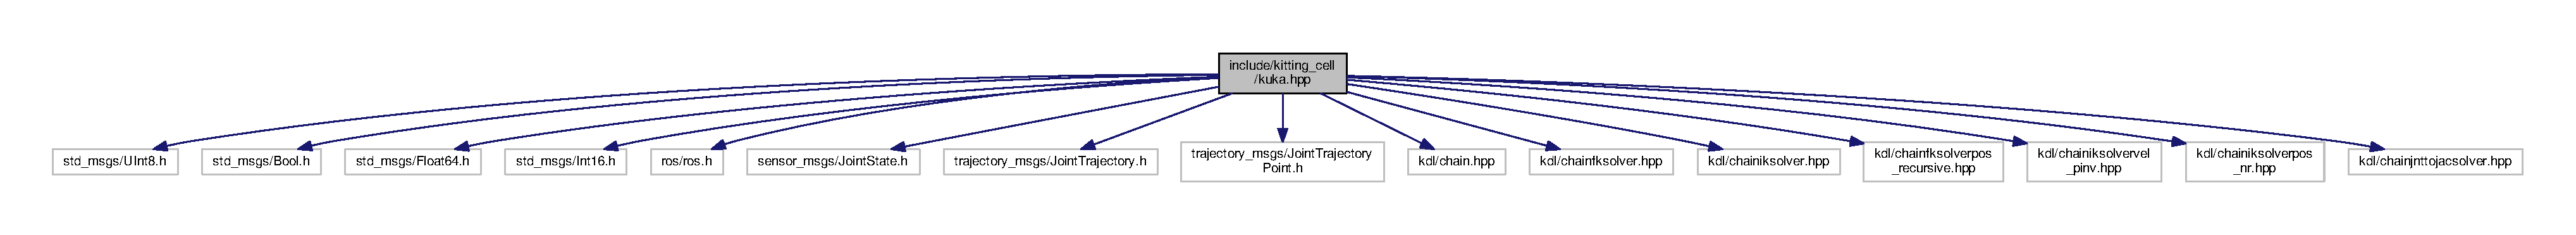
\includegraphics[width=350pt]{kuka_8hpp__incl}
\end{center}
\end{figure}
This graph shows which files directly or indirectly include this file\+:
\nopagebreak
\begin{figure}[H]
\begin{center}
\leavevmode
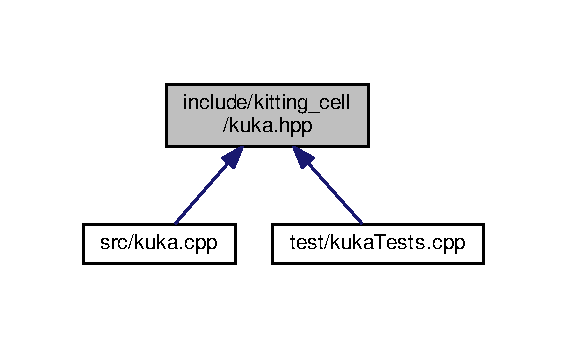
\includegraphics[width=272pt]{kuka_8hpp__dep__incl}
\end{center}
\end{figure}
\subsection*{Classes}
\begin{DoxyCompactItemize}
\item 
class \hyperlink{classkuka}{kuka}
\begin{DoxyCompactList}\small\item\em Class to calculate forward and inverse kinematics for K\+U\+KA I\+I\+WA. \end{DoxyCompactList}\end{DoxyCompactItemize}


\subsection{Detailed Description}
This file defines the methods for class \char`\"{}kuka\char`\"{} to control a K\+U\+KA I\+I\+WA manipulator using on I\+I\+W\+A\+\_\+\+S\+T\+A\+CK using O\+R\+O\+C\+OS K\+DL. 

\begin{DoxyAuthor}{Author}
Bharat Mathur \mbox{[}bharatm11\mbox{]} -\/ driver 

Royneal Rayess \mbox{[}royneal\mbox{]} -\/ navigator 
\end{DoxyAuthor}
\begin{DoxyDate}{Date}
27 Nov 2018 
\end{DoxyDate}
\begin{DoxyCopyright}{Copyright}
2018 Bharat Mathur, Royneal Rayess 
\end{DoxyCopyright}

\hypertarget{Perception_8hpp}{}\section{include/kitting\+\_\+cell/\+Perception.hpp File Reference}
\label{Perception_8hpp}\index{include/kitting\+\_\+cell/\+Perception.\+hpp@{include/kitting\+\_\+cell/\+Perception.\+hpp}}


This file defines the methods for class the \hyperlink{classPerception}{Perception} class. This class is responsible for detection and localizing red, green, and blue objects in the image which is read through a R\+OS topic.  


{\ttfamily \#include $<$ros/ros.\+h$>$}\\*
{\ttfamily \#include $<$cv\+\_\+bridge/cv\+\_\+bridge.\+h$>$}\\*
{\ttfamily \#include $<$image\+\_\+transport/image\+\_\+transport.\+h$>$}\\*
{\ttfamily \#include $<$string$>$}\\*
{\ttfamily \#include $<$vector$>$}\\*
{\ttfamily \#include $<$opencv2/highgui/highgui.\+hpp$>$}\\*
Include dependency graph for Perception.\+hpp\+:
\nopagebreak
\begin{figure}[H]
\begin{center}
\leavevmode
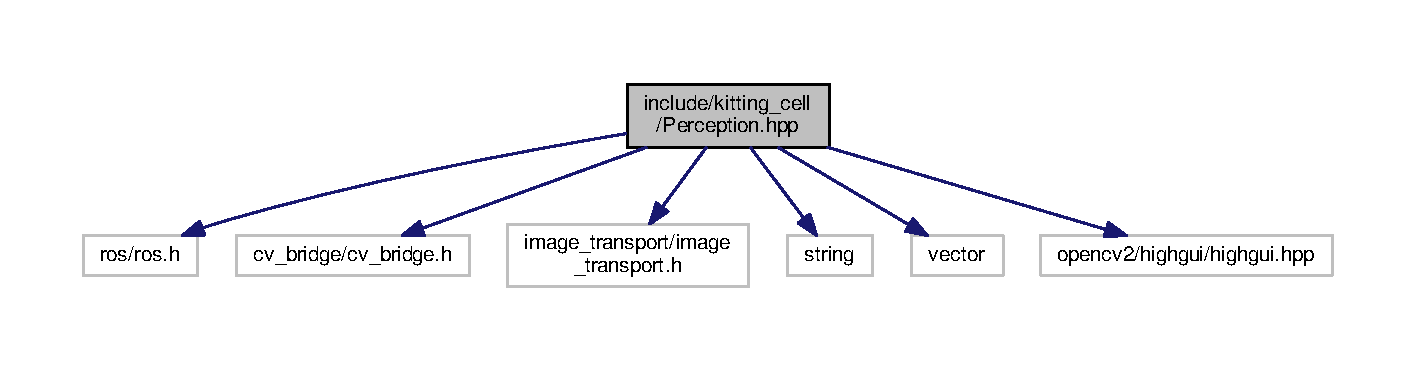
\includegraphics[width=350pt]{Perception_8hpp__incl}
\end{center}
\end{figure}
This graph shows which files directly or indirectly include this file\+:
\nopagebreak
\begin{figure}[H]
\begin{center}
\leavevmode
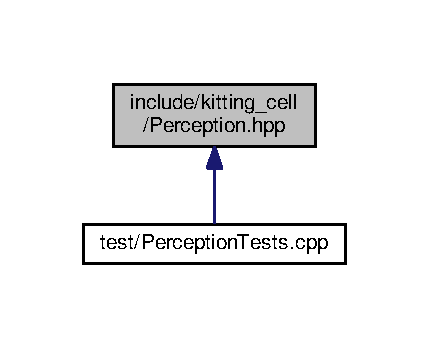
\includegraphics[width=206pt]{Perception_8hpp__dep__incl}
\end{center}
\end{figure}
\subsection*{Classes}
\begin{DoxyCompactItemize}
\item 
class \hyperlink{classPerception}{Perception}
\end{DoxyCompactItemize}


\subsection{Detailed Description}
This file defines the methods for class the \hyperlink{classPerception}{Perception} class. This class is responsible for detection and localizing red, green, and blue objects in the image which is read through a R\+OS topic. 

This file defines methods for detecting object colors and localizing them to provide the mainpulator with a pick target.

\begin{DoxyAuthor}{Author}
Bharat Mathur \mbox{[}bharatm11\mbox{]} -\/ driver 

Royneal Rayess \mbox{[}royneal\mbox{]} -\/ navigator 
\end{DoxyAuthor}
\begin{DoxyDate}{Date}
12 Dec 2018 
\end{DoxyDate}
\begin{DoxyCopyright}{Copyright}
2018 Bharat Mathur, Royneal Rayess 
\end{DoxyCopyright}

\hypertarget{Grip_8cpp}{}\section{src/\+Grip.cpp File Reference}
\label{Grip_8cpp}\index{src/\+Grip.\+cpp@{src/\+Grip.\+cpp}}


This file defines methods for the \hyperlink{classGrip}{Grip} class. This class is used to toggle the vacuum gripper on a manipulator.  


{\ttfamily \#include \char`\"{}Grip.\+hpp\char`\"{}}\\*
Include dependency graph for Grip.\+cpp\+:
\nopagebreak
\begin{figure}[H]
\begin{center}
\leavevmode
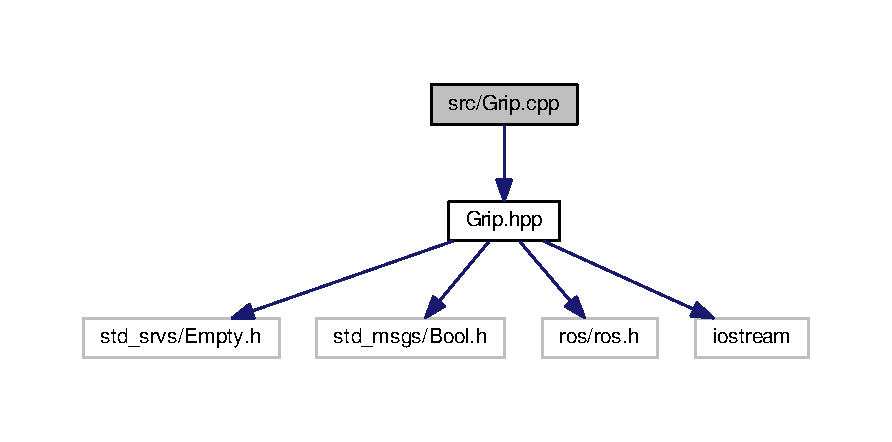
\includegraphics[width=350pt]{Grip_8cpp__incl}
\end{center}
\end{figure}


\subsection{Detailed Description}
This file defines methods for the \hyperlink{classGrip}{Grip} class. This class is used to toggle the vacuum gripper on a manipulator. 

\begin{DoxyAuthor}{Author}
Royneal Rayess \mbox{[}royneal\mbox{]} -\/ driver 

Bharat Mathur \mbox{[}bharatm11\mbox{]} -\/ navigator 
\end{DoxyAuthor}
\begin{DoxyDate}{Date}
15 Dec 2018 
\end{DoxyDate}
\begin{DoxyCopyright}{Copyright}
2018 Royneal Rayess, Bharat Mathur
\end{DoxyCopyright}
\begin{DoxyAuthor}{Author}
Bharat Mathur \mbox{[}bharatm11\mbox{]} -\/ driver 

Royneal Rayess \mbox{[}royneal\mbox{]} -\/ navigator 
\end{DoxyAuthor}
\begin{DoxyDate}{Date}
15 Dec 2018 
\end{DoxyDate}
\begin{DoxyCopyright}{Copyright}
2018 Bharat Mathur, Royneal Rayess 
\end{DoxyCopyright}

\hypertarget{kuka_8cpp}{}\section{src/kuka.cpp File Reference}
\label{kuka_8cpp}\index{src/kuka.\+cpp@{src/kuka.\+cpp}}


This file implements the methods for class \char`\"{}kuka\char`\"{} This class cpp file defines data members and methods applicable for class kuka to to control a K\+U\+KA I\+I\+WA manipulator using on I\+I\+W\+A\+\_\+\+S\+T\+A\+CK using O\+R\+O\+C\+OS K\+DL for forward and inverse kinematics.  


{\ttfamily \#include $<$std\+\_\+msgs/\+U\+Int8.\+h$>$}\\*
{\ttfamily \#include $<$std\+\_\+msgs/\+Bool.\+h$>$}\\*
{\ttfamily \#include $<$std\+\_\+msgs/\+Float64.\+h$>$}\\*
{\ttfamily \#include $<$std\+\_\+msgs/\+Int16.\+h$>$}\\*
{\ttfamily \#include $<$ros/ros.\+h$>$}\\*
{\ttfamily \#include $<$sensor\+\_\+msgs/\+Joint\+State.\+h$>$}\\*
{\ttfamily \#include $<$trajectory\+\_\+msgs/\+Joint\+Trajectory.\+h$>$}\\*
{\ttfamily \#include $<$trajectory\+\_\+msgs/\+Joint\+Trajectory\+Point.\+h$>$}\\*
{\ttfamily \#include $<$kdl/chain.\+hpp$>$}\\*
{\ttfamily \#include $<$kdl/chainfksolver.\+hpp$>$}\\*
{\ttfamily \#include $<$kdl/chainiksolver.\+hpp$>$}\\*
{\ttfamily \#include $<$kdl/chainfksolverpos\+\_\+recursive.\+hpp$>$}\\*
{\ttfamily \#include $<$kdl/chainiksolvervel\+\_\+pinv.\+hpp$>$}\\*
{\ttfamily \#include $<$kdl/chainiksolverpos\+\_\+nr.\+hpp$>$}\\*
{\ttfamily \#include $<$kdl/chainjnttojacsolver.\+hpp$>$}\\*
{\ttfamily \#include \char`\"{}kuka.\+hpp\char`\"{}}\\*
Include dependency graph for kuka.\+cpp\+:
\nopagebreak
\begin{figure}[H]
\begin{center}
\leavevmode
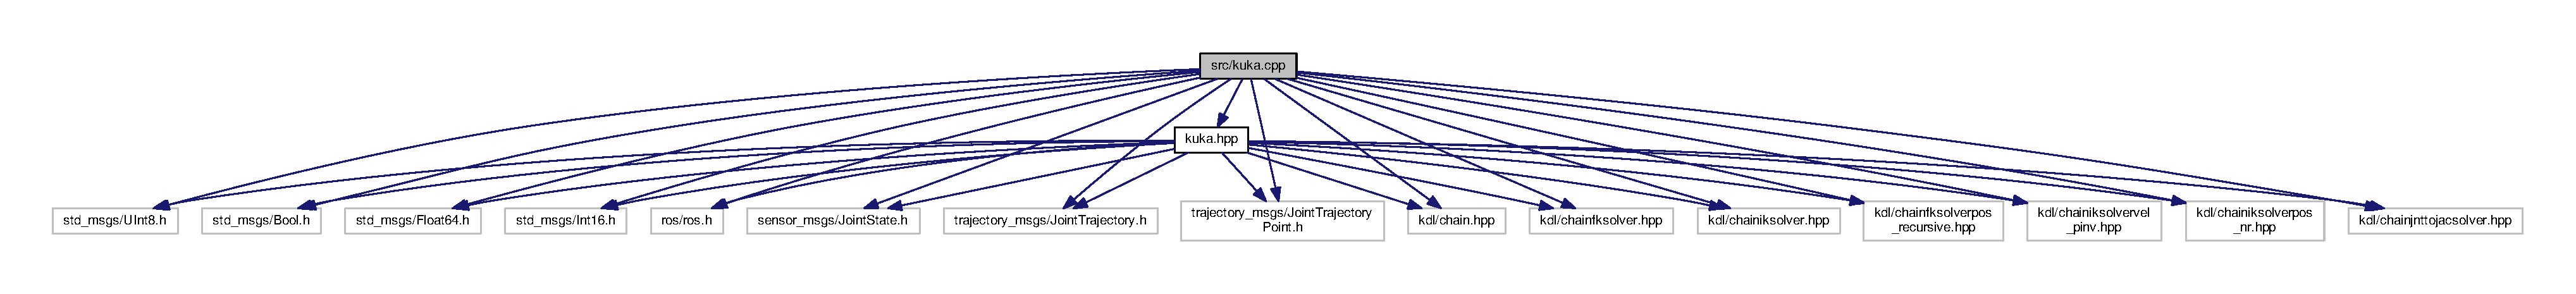
\includegraphics[width=350pt]{kuka_8cpp__incl}
\end{center}
\end{figure}


\subsection{Detailed Description}
This file implements the methods for class \char`\"{}kuka\char`\"{} This class cpp file defines data members and methods applicable for class kuka to to control a K\+U\+KA I\+I\+WA manipulator using on I\+I\+W\+A\+\_\+\+S\+T\+A\+CK using O\+R\+O\+C\+OS K\+DL for forward and inverse kinematics. 

\begin{DoxyAuthor}{Author}
Bharat Mathur \mbox{[}bharatm11\mbox{]} -\/ driver 

Royneal Rayess \mbox{[}royneal\mbox{]} -\/ navigator 
\end{DoxyAuthor}
\begin{DoxyDate}{Date}
27 Nov 2018 
\end{DoxyDate}
\begin{DoxyCopyright}{Copyright}
2018 Bharat Mathur, Royneal Rayess 
\end{DoxyCopyright}

\hypertarget{GripTests_8cpp}{}\section{test/\+Grip\+Tests.cpp File Reference}
\label{GripTests_8cpp}\index{test/\+Grip\+Tests.\+cpp@{test/\+Grip\+Tests.\+cpp}}


This file defines the rostests and getests for \hyperlink{classGrip}{Grip} class.  


{\ttfamily \#include $<$gtest/gtest.\+h$>$}\\*
{\ttfamily \#include \char`\"{}Grip.\+hpp\char`\"{}}\\*
Include dependency graph for Grip\+Tests.\+cpp\+:
\nopagebreak
\begin{figure}[H]
\begin{center}
\leavevmode
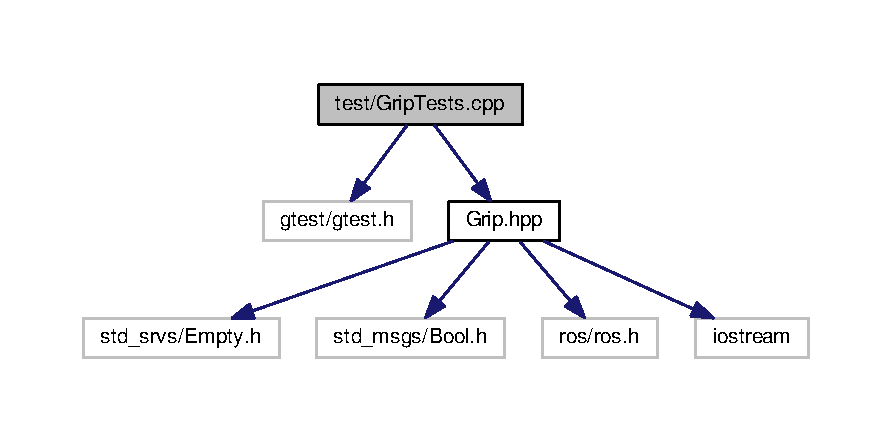
\includegraphics[width=350pt]{GripTests_8cpp__incl}
\end{center}
\end{figure}
\subsection*{Functions}
\begin{DoxyCompactItemize}
\item 
{\bfseries T\+E\+ST} (Grip\+Test, test\+Get\+Gripper\+State)\hypertarget{GripTests_8cpp_a7eb7c5095a218d53411f8b148b420456}{}\label{GripTests_8cpp_a7eb7c5095a218d53411f8b148b420456}

\end{DoxyCompactItemize}


\subsection{Detailed Description}
This file defines the rostests and getests for \hyperlink{classGrip}{Grip} class. 

G\+NU L\+E\+S\+S\+ER G\+E\+N\+E\+R\+AL P\+U\+B\+L\+IC L\+I\+C\+E\+N\+SE Version 3, 29 June 2007

Copyright (C) 2007 Free Software Foundation, Inc. \href{https://fsf.org/}{\tt https\+://fsf.\+org/} Everyone is permitted to copy and distribute verbatim copies of this license document, but changing it is not allowed.

This version of the G\+NU Lesser General Public License incorporates the terms and conditions of version 3 of the G\+NU General Public License, supplemented by the additional permissions listed below.

0. Additional Definitions.

As used herein, \char`\"{}this License\char`\"{} refers to version 3 of the G\+NU Lesser General Public License, and the \char`\"{}\+G\+N\+U G\+P\+L\char`\"{} refers to version 3 of the G\+NU General Public License.

\char`\"{}\+The Library\char`\"{} refers to a covered work governed by this License, other than an Application or a Combined Work as defined below.

An \char`\"{}\+Application\char`\"{} is any work that makes use of an interface provided by the Library, but which is not otherwise based on the Library. Defining a subclass of a class defined by the Library is deemed a mode of using an interface provided by the Library.

A \char`\"{}\+Combined Work\char`\"{} is a work produced by combining or linking an Application with the Library. The particular version of the Library with which the Combined Work was made is also called the \char`\"{}\+Linked
\+Version\char`\"{}.

The \char`\"{}\+Minimal Corresponding Source\char`\"{} for a Combined Work means the Corresponding Source for the Combined Work, excluding any source code for portions of the Combined Work that, considered in isolation, are based on the Application, and not on the Linked Version.

The \char`\"{}\+Corresponding Application Code\char`\"{} for a Combined Work means the object code and/or source code for the Application, including any data and utility programs needed for reproducing the Combined Work from the Application, but excluding the System Libraries of the Combined Work.


\begin{DoxyEnumerate}
\item Exception to Section 3 of the G\+NU G\+PL.
\end{DoxyEnumerate}

You may convey a covered work under sections 3 and 4 of this License without being bound by section 3 of the G\+NU G\+PL.


\begin{DoxyEnumerate}
\item Conveying Modified Versions.
\end{DoxyEnumerate}

If you modify a copy of the Library, and, in your modifications, a facility refers to a function or data to be supplied by an Application that uses the facility (other than as an argument passed when the facility is invoked), then you may convey a copy of the modified version\+:

a) under this License, provided that you make a good faith effort to ensure that, in the event an Application does not supply the function or data, the facility still operates, and performs whatever part of its purpose remains meaningful, or

b) under the G\+NU G\+PL, with none of the additional permissions of this License applicable to that copy.


\begin{DoxyEnumerate}
\item Object Code Incorporating Material from Library Header Files.
\end{DoxyEnumerate}

The object code form of an Application may incorporate material from a header file that is part of the Library. You may convey such object code under terms of your choice, provided that, if the incorporated material is not limited to numerical parameters, data structure layouts and accessors, or small macros, inline functions and templates (ten or fewer lines in length), you do both of the following\+:

a) Give prominent notice with each copy of the object code that the Library is used in it and that the Library and its use are covered by this License.

b) Accompany the object code with a copy of the G\+NU G\+PL and this license document.


\begin{DoxyEnumerate}
\item Combined Works.
\end{DoxyEnumerate}

You may convey a Combined Work under terms of your choice that, taken together, effectively do not restrict modification of the portions of the Library contained in the Combined Work and reverse engineering for debugging such modifications, if you also do each of the following\+:

a) Give prominent notice with each copy of the Combined Work that the Library is used in it and that the Library and its use are covered by this License.

b) Accompany the Combined Work with a copy of the G\+NU G\+PL and this license document.

c) For a Combined Work that displays copyright notices during execution, include the copyright notice for the Library among these notices, as well as a reference directing the user to the copies of the G\+NU G\+PL and this license document.

d) Do one of the following\+: \begin{DoxyVerb}0) Convey the Minimal Corresponding Source under the terms of this
License, and the Corresponding Application Code in a form
suitable for, and under terms that permit, the user to
recombine or relink the Application with a modified version of
the Linked Version to produce a modified Combined Work, in the
manner specified by section 6 of the GNU GPL for conveying
Corresponding Source.

1) Use a suitable shared library mechanism for linking with the
Library.  A suitable mechanism is one that (a) uses at run time
a copy of the Library already present on the user's computer
system, and (b) will operate properly with a modified version
of the Library that is interface-compatible with the Linked
Version.
\end{DoxyVerb}


e) Provide Installation Information, but only if you would otherwise be required to provide such information under section 6 of the G\+NU G\+PL, and only to the extent that such information is necessary to install and execute a modified version of the Combined Work produced by recombining or relinking the Application with a modified version of the Linked Version. (If you use option 4d0, the Installation Information must accompany the Minimal Corresponding Source and Corresponding Application Code. If you use option 4d1, you must provide the Installation Information in the manner specified by section 6 of the G\+NU G\+PL for conveying Corresponding Source.)


\begin{DoxyEnumerate}
\item Combined Libraries.
\end{DoxyEnumerate}

You may place library facilities that are a work based on the Library side by side in a single library together with other library facilities that are not Applications and are not covered by this License, and convey such a combined library under terms of your choice, if you do both of the following\+:

a) Accompany the combined library with a copy of the same work based on the Library, uncombined with any other library facilities, conveyed under the terms of this License.

b) Give prominent notice with the combined library that part of it is a work based on the Library, and explaining where to find the accompanying uncombined form of the same work.


\begin{DoxyEnumerate}
\item Revised Versions of the G\+NU Lesser General Public License.
\end{DoxyEnumerate}

The Free Software Foundation may publish revised and/or new versions of the G\+NU Lesser General Public License from time to time. Such new versions will be similar in spirit to the present version, but may differ in detail to address new problems or concerns.

Each version is given a distinguishing version number. If the Library as you received it specifies that a certain numbered version of the G\+NU Lesser General Public License \char`\"{}or any later version\char`\"{} applies to it, you have the option of following the terms and conditions either of that published version or of any later version published by the Free Software Foundation. If the Library as you received it does not specify a version number of the G\+NU Lesser General Public License, you may choose any version of the G\+NU Lesser General Public License ever published by the Free Software Foundation.

If the Library as you received it specifies that a proxy can decide whether future versions of the G\+NU Lesser General Public License shall apply, that proxy\textquotesingle{}s public statement of acceptance of any version is permanent authorization for you to choose that version for the Library.

\begin{DoxyAuthor}{Author}
Bharat Mathur \mbox{[}bharatm11\mbox{]} -\/ driver 

Royneal Rayess \mbox{[}royneal\mbox{]} -\/ navigator 
\end{DoxyAuthor}
\begin{DoxyDate}{Date}
15 Dec 2018 
\end{DoxyDate}
\begin{DoxyCopyright}{Copyright}
2018 Bharat Mathur 
\end{DoxyCopyright}

\hypertarget{kukaTests_8cpp}{}\section{test/kuka\+Tests.cpp File Reference}
\label{kukaTests_8cpp}\index{test/kuka\+Tests.\+cpp@{test/kuka\+Tests.\+cpp}}


This is the file for testing the methods of the kuka class.  


{\ttfamily \#include $<$gtest/gtest.\+h$>$}\\*
{\ttfamily \#include $<$std\+\_\+msgs/\+U\+Int8.\+h$>$}\\*
{\ttfamily \#include $<$std\+\_\+msgs/\+Bool.\+h$>$}\\*
{\ttfamily \#include $<$std\+\_\+msgs/\+Float64.\+h$>$}\\*
{\ttfamily \#include $<$std\+\_\+msgs/\+Int16.\+h$>$}\\*
{\ttfamily \#include $<$ros/ros.\+h$>$}\\*
{\ttfamily \#include $<$sensor\+\_\+msgs/\+Joint\+State.\+h$>$}\\*
{\ttfamily \#include $<$trajectory\+\_\+msgs/\+Joint\+Trajectory.\+h$>$}\\*
{\ttfamily \#include $<$trajectory\+\_\+msgs/\+Joint\+Trajectory\+Point.\+h$>$}\\*
{\ttfamily \#include $<$kdl/chain.\+hpp$>$}\\*
{\ttfamily \#include $<$kdl/chainfksolver.\+hpp$>$}\\*
{\ttfamily \#include $<$kdl/chainiksolver.\+hpp$>$}\\*
{\ttfamily \#include $<$kdl/chainfksolverpos\+\_\+recursive.\+hpp$>$}\\*
{\ttfamily \#include $<$kdl/chainiksolvervel\+\_\+pinv.\+hpp$>$}\\*
{\ttfamily \#include $<$kdl/chainiksolverpos\+\_\+nr.\+hpp$>$}\\*
{\ttfamily \#include $<$kdl/chainjnttojacsolver.\+hpp$>$}\\*
{\ttfamily \#include \char`\"{}kuka.\+hpp\char`\"{}}\\*
Include dependency graph for kuka\+Tests.\+cpp\+:
\nopagebreak
\begin{figure}[H]
\begin{center}
\leavevmode
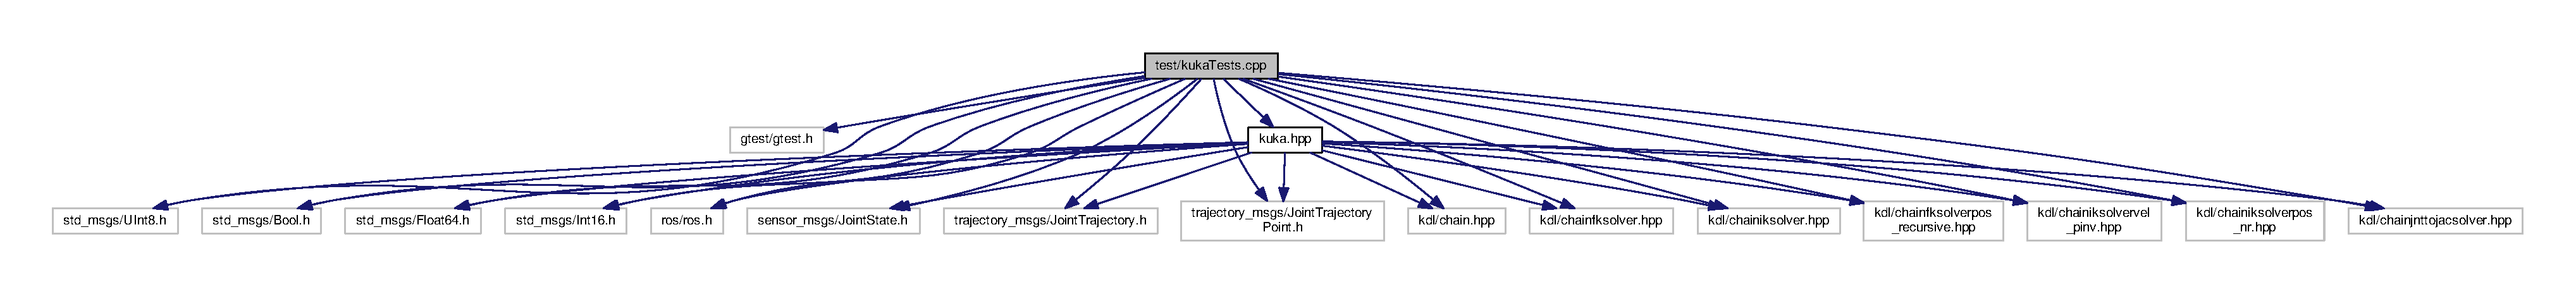
\includegraphics[width=350pt]{kukaTests_8cpp__incl}
\end{center}
\end{figure}
\subsection*{Functions}
\begin{DoxyCompactItemize}
\item 
{\bfseries T\+E\+ST} (initialize\+Trajectory\+Point\+Test, Check\+Joint\+Names)\hypertarget{kukaTests_8cpp_a8a274457ca8880526287b3687f30f441}{}\label{kukaTests_8cpp_a8a274457ca8880526287b3687f30f441}

\item 
{\bfseries T\+E\+ST} (initialize\+Trajectory\+Point\+Test, Check\+Trajectoryheader)\hypertarget{kukaTests_8cpp_a502ab2f50aefec1289421a347bbb2e96}{}\label{kukaTests_8cpp_a502ab2f50aefec1289421a347bbb2e96}

\item 
{\bfseries T\+E\+ST} (initialize\+Home\+Pos\+Test, Check\+Home\+Pos)\hypertarget{kukaTests_8cpp_aaa8d18f9665d1b9fb24da7584c1ca5ae}{}\label{kukaTests_8cpp_aaa8d18f9665d1b9fb24da7584c1ca5ae}

\item 
{\bfseries T\+E\+ST} (initialize\+Joints\+Sub\+Test, Check\+Joint\+Sub)\hypertarget{kukaTests_8cpp_aac86c8b2e040e4c3ad666871f942893c}{}\label{kukaTests_8cpp_aac86c8b2e040e4c3ad666871f942893c}

\item 
{\bfseries T\+E\+ST} (initialize\+Joints\+K\+D\+L\+Test, Check\+Joints\+K\+DL)\hypertarget{kukaTests_8cpp_a24c2f7311754d601fe6db831339f9383}{}\label{kukaTests_8cpp_a24c2f7311754d601fe6db831339f9383}

\item 
{\bfseries T\+E\+ST} (make\+Chain\+Test, Check\+Chain)\hypertarget{kukaTests_8cpp_a94ccf49ee0ad472534ba17b006709b72}{}\label{kukaTests_8cpp_a94ccf49ee0ad472534ba17b006709b72}

\item 
{\bfseries T\+E\+ST} (Evaluate\+Kinematics, Check\+FK)\hypertarget{kukaTests_8cpp_a489f669b22c591c4ddbc30735daacac4}{}\label{kukaTests_8cpp_a489f669b22c591c4ddbc30735daacac4}

\item 
{\bfseries T\+E\+ST} (Get\+Joint\+Numbers\+Test, Checkget\+Joint\+Nums)\hypertarget{kukaTests_8cpp_a3057258772412cab360a76dcc4bec723}{}\label{kukaTests_8cpp_a3057258772412cab360a76dcc4bec723}

\item 
{\bfseries T\+E\+ST} (normalize\+Points\+Test, Checknormalized\+Points)\hypertarget{kukaTests_8cpp_a944f11fd13e20ddcaac1fdb9b0fcc8e2}{}\label{kukaTests_8cpp_a944f11fd13e20ddcaac1fdb9b0fcc8e2}

\item 
{\bfseries T\+E\+ST} (Evaluate\+Kinematics\+Test, Check\+IK)\hypertarget{kukaTests_8cpp_abc0a9c9322bdf8724c79076cd0992f43}{}\label{kukaTests_8cpp_abc0a9c9322bdf8724c79076cd0992f43}

\item 
{\bfseries T\+E\+ST} (drive\+Robot\+Test, names)\hypertarget{kukaTests_8cpp_ad06a96d970b49f32fc6aa0057716e596}{}\label{kukaTests_8cpp_ad06a96d970b49f32fc6aa0057716e596}

\item 
{\bfseries T\+E\+ST} (drive\+Robot\+Test, properties)\hypertarget{kukaTests_8cpp_a1e34471f9cc0b53f308e5b814ef430cf}{}\label{kukaTests_8cpp_a1e34471f9cc0b53f308e5b814ef430cf}

\item 
{\bfseries T\+E\+ST} (return\+Curr\+Joints\+Test, joints)\hypertarget{kukaTests_8cpp_a136adebcba5438a17104161c8a5f96c4}{}\label{kukaTests_8cpp_a136adebcba5438a17104161c8a5f96c4}

\end{DoxyCompactItemize}


\subsection{Detailed Description}
This is the file for testing the methods of the kuka class. 

G\+NU L\+E\+S\+S\+ER G\+E\+N\+E\+R\+AL P\+U\+B\+L\+IC L\+I\+C\+E\+N\+SE Version 3, 29 June 2007

Copyright (C) 2007 Free Software Foundation, Inc. \href{https://fsf.org/}{\tt https\+://fsf.\+org/} Everyone is permitted to copy and distribute verbatim copies of this license document, but changing it is not allowed.

This version of the G\+NU Lesser General Public License incorporates the terms and conditions of version 3 of the G\+NU General Public License, supplemented by the additional permissions listed below.

0. Additional Definitions.

As used herein, \char`\"{}this License\char`\"{} refers to version 3 of the G\+NU Lesser General Public License, and the \char`\"{}\+G\+N\+U G\+P\+L\char`\"{} refers to version 3 of the G\+NU General Public License.

\char`\"{}\+The Library\char`\"{} refers to a covered work governed by this License, other than an Application or a Combined Work as defined below.

An \char`\"{}\+Application\char`\"{} is any work that makes use of an interface provided by the Library, but which is not otherwise based on the Library. Defining a subclass of a class defined by the Library is deemed a mode of using an interface provided by the Library.

A \char`\"{}\+Combined Work\char`\"{} is a work produced by combining or linking an Application with the Library. The particular version of the Library with which the Combined Work was made is also called the \char`\"{}\+Linked
\+Version\char`\"{}.

The \char`\"{}\+Minimal Corresponding Source\char`\"{} for a Combined Work means the Corresponding Source for the Combined Work, excluding any source code for portions of the Combined Work that, considered in isolation, are based on the Application, and not on the Linked Version.

The \char`\"{}\+Corresponding Application Code\char`\"{} for a Combined Work means the object code and/or source code for the Application, including any data and utility programs needed for reproducing the Combined Work from the Application, but excluding the System Libraries of the Combined Work.


\begin{DoxyEnumerate}
\item Exception to Section 3 of the G\+NU G\+PL.
\end{DoxyEnumerate}

You may convey a covered work under sections 3 and 4 of this License without being bound by section 3 of the G\+NU G\+PL.


\begin{DoxyEnumerate}
\item Conveying Modified Versions.
\end{DoxyEnumerate}

If you modify a copy of the Library, and, in your modifications, a facility refers to a function or data to be supplied by an Application that uses the facility (other than as an argument passed when the facility is invoked), then you may convey a copy of the modified version\+:

a) under this License, provided that you make a good faith effort to ensure that, in the event an Application does not supply the function or data, the facility still operates, and performs whatever part of its purpose remains meaningful, or

b) under the G\+NU G\+PL, with none of the additional permissions of this License applicable to that copy.


\begin{DoxyEnumerate}
\item Object Code Incorporating Material from Library Header Files.
\end{DoxyEnumerate}

The object code form of an Application may incorporate material from a header file that is part of the Library. You may convey such object code under terms of your choice, provided that, if the incorporated material is not limited to numerical parameters, data structure layouts and accessors, or small macros, inline functions and templates (ten or fewer lines in length), you do both of the following\+:

a) Give prominent notice with each copy of the object code that the Library is used in it and that the Library and its use are covered by this License.

b) Accompany the object code with a copy of the G\+NU G\+PL and this license document.


\begin{DoxyEnumerate}
\item Combined Works.
\end{DoxyEnumerate}

You may convey a Combined Work under terms of your choice that, taken together, effectively do not restrict modification of the portions of the Library contained in the Combined Work and reverse engineering for debugging such modifications, if you also do each of the following\+:

a) Give prominent notice with each copy of the Combined Work that the Library is used in it and that the Library and its use are covered by this License.

b) Accompany the Combined Work with a copy of the G\+NU G\+PL and this license document.

c) For a Combined Work that displays copyright notices during execution, include the copyright notice for the Library among these notices, as well as a reference directing the user to the copies of the G\+NU G\+PL and this license document.

d) Do one of the following\+: \begin{DoxyVerb}0) Convey the Minimal Corresponding Source under the terms of this
License, and the Corresponding Application Code in a form
suitable for, and under terms that permit, the user to
recombine or relink the Application with a modified version of
the Linked Version to produce a modified Combined Work, in the
manner specified by section 6 of the GNU GPL for conveying
Corresponding Source.

1) Use a suitable shared library mechanism for linking with the
Library.  A suitable mechanism is one that (a) uses at run time
a copy of the Library already present on the user's computer
system, and (b) will operate properly with a modified version
of the Library that is interface-compatible with the Linked
Version.
\end{DoxyVerb}


e) Provide Installation Information, but only if you would otherwise be required to provide such information under section 6 of the G\+NU G\+PL, and only to the extent that such information is necessary to install and execute a modified version of the Combined Work produced by recombining or relinking the Application with a modified version of the Linked Version. (If you use option 4d0, the Installation Information must accompany the Minimal Corresponding Source and Corresponding Application Code. If you use option 4d1, you must provide the Installation Information in the manner specified by section 6 of the G\+NU G\+PL for conveying Corresponding Source.)


\begin{DoxyEnumerate}
\item Combined Libraries.
\end{DoxyEnumerate}

You may place library facilities that are a work based on the Library side by side in a single library together with other library facilities that are not Applications and are not covered by this License, and convey such a combined library under terms of your choice, if you do both of the following\+:

a) Accompany the combined library with a copy of the same work based on the Library, uncombined with any other library facilities, conveyed under the terms of this License.

b) Give prominent notice with the combined library that part of it is a work based on the Library, and explaining where to find the accompanying uncombined form of the same work.


\begin{DoxyEnumerate}
\item Revised Versions of the G\+NU Lesser General Public License.
\end{DoxyEnumerate}

The Free Software Foundation may publish revised and/or new versions of the G\+NU Lesser General Public License from time to time. Such new versions will be similar in spirit to the present version, but may differ in detail to address new problems or concerns.

Each version is given a distinguishing version number. If the Library as you received it specifies that a certain numbered version of the G\+NU Lesser General Public License \char`\"{}or any later version\char`\"{} applies to it, you have the option of following the terms and conditions either of that published version or of any later version published by the Free Software Foundation. If the Library as you received it does not specify a version number of the G\+NU Lesser General Public License, you may choose any version of the G\+NU Lesser General Public License ever published by the Free Software Foundation.

If the Library as you received it specifies that a proxy can decide whether future versions of the G\+NU Lesser General Public License shall apply, that proxy\textquotesingle{}s public statement of acceptance of any version is permanent authorization for you to choose that version for the Library.

\begin{DoxyAuthor}{Author}
Royneal Rayess \mbox{[}royneal\mbox{]} -\/ driver 

Bharat Mathur \mbox{[}bharatm11\mbox{]} -\/ navigator 
\end{DoxyAuthor}
\begin{DoxyDate}{Date}
13 Dec 2018 
\end{DoxyDate}
\begin{DoxyCopyright}{Copyright}
2018 Royneal Rayess 
\end{DoxyCopyright}

\hypertarget{PerceptionTests_8cpp}{}\section{test/\+Perception\+Tests.cpp File Reference}
\label{PerceptionTests_8cpp}\index{test/\+Perception\+Tests.\+cpp@{test/\+Perception\+Tests.\+cpp}}


This is the file for testing the methods of the \hyperlink{classPerception}{Perception} class.  


{\ttfamily \#include $<$gtest/gtest.\+h$>$}\\*
{\ttfamily \#include $<$ros/ros.\+h$>$}\\*
{\ttfamily \#include $<$image\+\_\+transport/image\+\_\+transport.\+h$>$}\\*
{\ttfamily \#include $<$cv\+\_\+bridge/cv\+\_\+bridge.\+h$>$}\\*
{\ttfamily \#include $<$sensor\+\_\+msgs/image\+\_\+encodings.\+h$>$}\\*
{\ttfamily \#include $<$opencv2/imgproc/imgproc.\+hpp$>$}\\*
{\ttfamily \#include $<$opencv2/highgui/highgui.\+hpp$>$}\\*
{\ttfamily \#include \char`\"{}Perception.\+hpp\char`\"{}}\\*
Include dependency graph for Perception\+Tests.\+cpp\+:
\nopagebreak
\begin{figure}[H]
\begin{center}
\leavevmode
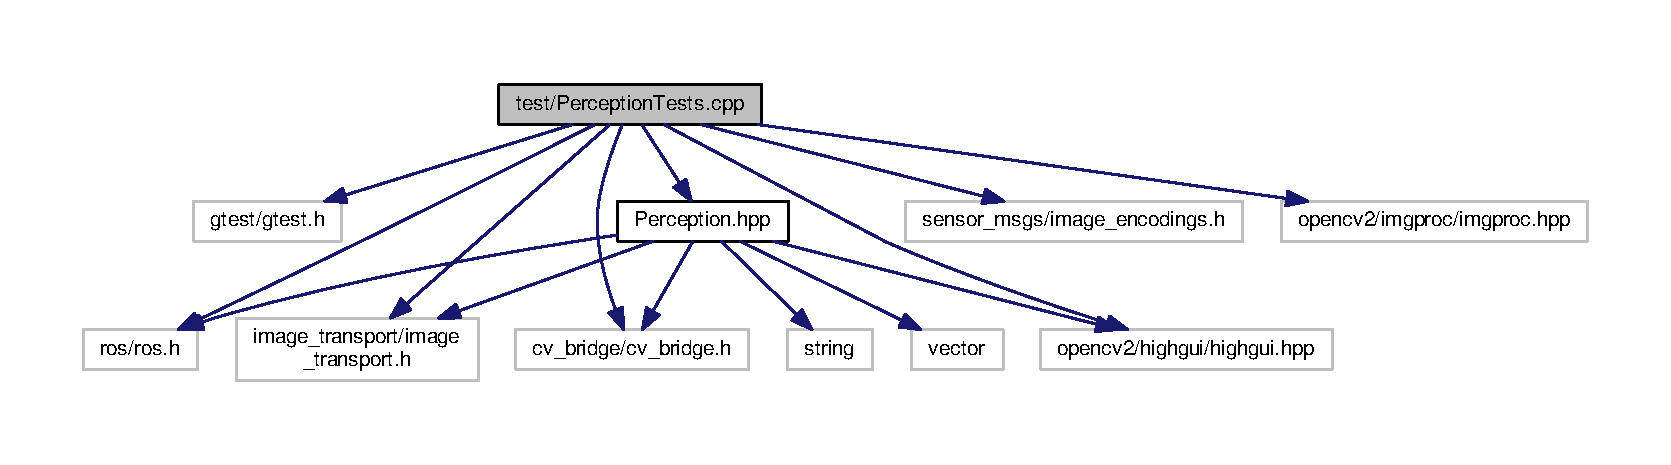
\includegraphics[width=350pt]{PerceptionTests_8cpp__incl}
\end{center}
\end{figure}
\subsection*{Functions}
\begin{DoxyCompactItemize}
\item 
{\bfseries T\+E\+ST} (color\+Thresholder\+Test, Check\+Return\+Output)\hypertarget{PerceptionTests_8cpp_ad743064fc41aa7317d913725cca7a6cd}{}\label{PerceptionTests_8cpp_ad743064fc41aa7317d913725cca7a6cd}

\end{DoxyCompactItemize}


\subsection{Detailed Description}
This is the file for testing the methods of the \hyperlink{classPerception}{Perception} class. 

G\+NU L\+E\+S\+S\+ER G\+E\+N\+E\+R\+AL P\+U\+B\+L\+IC L\+I\+C\+E\+N\+SE Version 3, 29 June 2007

Copyright (C) 2007 Free Software Foundation, Inc. \href{https://fsf.org/}{\tt https\+://fsf.\+org/} Everyone is permitted to copy and distribute verbatim copies of this license document, but changing it is not allowed.

This version of the G\+NU Lesser General Public License incorporates the terms and conditions of version 3 of the G\+NU General Public License, supplemented by the additional permissions listed below.

0. Additional Definitions.

As used herein, \char`\"{}this License\char`\"{} refers to version 3 of the G\+NU Lesser General Public License, and the \char`\"{}\+G\+N\+U G\+P\+L\char`\"{} refers to version 3 of the G\+NU General Public License.

\char`\"{}\+The Library\char`\"{} refers to a covered work governed by this License, other than an Application or a Combined Work as defined below.

An \char`\"{}\+Application\char`\"{} is any work that makes use of an interface provided by the Library, but which is not otherwise based on the Library. Defining a subclass of a class defined by the Library is deemed a mode of using an interface provided by the Library.

A \char`\"{}\+Combined Work\char`\"{} is a work produced by combining or linking an Application with the Library. The particular version of the Library with which the Combined Work was made is also called the \char`\"{}\+Linked
\+Version\char`\"{}.

The \char`\"{}\+Minimal Corresponding Source\char`\"{} for a Combined Work means the Corresponding Source for the Combined Work, excluding any source code for portions of the Combined Work that, considered in isolation, are based on the Application, and not on the Linked Version.

The \char`\"{}\+Corresponding Application Code\char`\"{} for a Combined Work means the object code and/or source code for the Application, including any data and utility programs needed for reproducing the Combined Work from the Application, but excluding the System Libraries of the Combined Work.


\begin{DoxyEnumerate}
\item Exception to Section 3 of the G\+NU G\+PL.
\end{DoxyEnumerate}

You may convey a covered work under sections 3 and 4 of this License without being bound by section 3 of the G\+NU G\+PL.


\begin{DoxyEnumerate}
\item Conveying Modified Versions.
\end{DoxyEnumerate}

If you modify a copy of the Library, and, in your modifications, a facility refers to a function or data to be supplied by an Application that uses the facility (other than as an argument passed when the facility is invoked), then you may convey a copy of the modified version\+:

a) under this License, provided that you make a good faith effort to ensure that, in the event an Application does not supply the function or data, the facility still operates, and performs whatever part of its purpose remains meaningful, or

b) under the G\+NU G\+PL, with none of the additional permissions of this License applicable to that copy.


\begin{DoxyEnumerate}
\item Object Code Incorporating Material from Library Header Files.
\end{DoxyEnumerate}

The object code form of an Application may incorporate material from a header file that is part of the Library. You may convey such object code under terms of your choice, provided that, if the incorporated material is not limited to numerical parameters, data structure layouts and accessors, or small macros, inline functions and templates (ten or fewer lines in length), you do both of the following\+:

a) Give prominent notice with each copy of the object code that the Library is used in it and that the Library and its use are covered by this License.

b) Accompany the object code with a copy of the G\+NU G\+PL and this license document.


\begin{DoxyEnumerate}
\item Combined Works.
\end{DoxyEnumerate}

You may convey a Combined Work under terms of your choice that, taken together, effectively do not restrict modification of the portions of the Library contained in the Combined Work and reverse engineering for debugging such modifications, if you also do each of the following\+:

a) Give prominent notice with each copy of the Combined Work that the Library is used in it and that the Library and its use are covered by this License.

b) Accompany the Combined Work with a copy of the G\+NU G\+PL and this license document.

c) For a Combined Work that displays copyright notices during execution, include the copyright notice for the Library among these notices, as well as a reference directing the user to the copies of the G\+NU G\+PL and this license document.

d) Do one of the following\+: \begin{DoxyVerb}0) Convey the Minimal Corresponding Source under the terms of this
License, and the Corresponding Application Code in a form
suitable for, and under terms that permit, the user to
recombine or relink the Application with a modified version of
the Linked Version to produce a modified Combined Work, in the
manner specified by section 6 of the GNU GPL for conveying
Corresponding Source.

1) Use a suitable shared library mechanism for linking with the
Library.  A suitable mechanism is one that (a) uses at run time
a copy of the Library already present on the user's computer
system, and (b) will operate properly with a modified version
of the Library that is interface-compatible with the Linked
Version.
\end{DoxyVerb}


e) Provide Installation Information, but only if you would otherwise be required to provide such information under section 6 of the G\+NU G\+PL, and only to the extent that such information is necessary to install and execute a modified version of the Combined Work produced by recombining or relinking the Application with a modified version of the Linked Version. (If you use option 4d0, the Installation Information must accompany the Minimal Corresponding Source and Corresponding Application Code. If you use option 4d1, you must provide the Installation Information in the manner specified by section 6 of the G\+NU G\+PL for conveying Corresponding Source.)


\begin{DoxyEnumerate}
\item Combined Libraries.
\end{DoxyEnumerate}

You may place library facilities that are a work based on the Library side by side in a single library together with other library facilities that are not Applications and are not covered by this License, and convey such a combined library under terms of your choice, if you do both of the following\+:

a) Accompany the combined library with a copy of the same work based on the Library, uncombined with any other library facilities, conveyed under the terms of this License.

b) Give prominent notice with the combined library that part of it is a work based on the Library, and explaining where to find the accompanying uncombined form of the same work.


\begin{DoxyEnumerate}
\item Revised Versions of the G\+NU Lesser General Public License.
\end{DoxyEnumerate}

The Free Software Foundation may publish revised and/or new versions of the G\+NU Lesser General Public License from time to time. Such new versions will be similar in spirit to the present version, but may differ in detail to address new problems or concerns.

Each version is given a distinguishing version number. If the Library as you received it specifies that a certain numbered version of the G\+NU Lesser General Public License \char`\"{}or any later version\char`\"{} applies to it, you have the option of following the terms and conditions either of that published version or of any later version published by the Free Software Foundation. If the Library as you received it does not specify a version number of the G\+NU Lesser General Public License, you may choose any version of the G\+NU Lesser General Public License ever published by the Free Software Foundation.

If the Library as you received it specifies that a proxy can decide whether future versions of the G\+NU Lesser General Public License shall apply, that proxy\textquotesingle{}s public statement of acceptance of any version is permanent authorization for you to choose that version for the Library.

\begin{DoxyAuthor}{Author}
Bharat Mathur \mbox{[}bharatm11\mbox{]} -\/ navigator 

Royneal Rayess \mbox{[}royneal\mbox{]} -\/ driver 
\end{DoxyAuthor}
\begin{DoxyDate}{Date}
13 Dec 2018 
\end{DoxyDate}
\begin{DoxyCopyright}{Copyright}
2018 Bharat Mathur 
\end{DoxyCopyright}

%--- End generated contents ---

% Index
\backmatter
\newpage
\phantomsection
\clearemptydoublepage
\addcontentsline{toc}{chapter}{Index}
\printindex

\end{document}
